\documentclass[conference]{IEEEtran}
\usepackage[utf8]{inputenc}
\usepackage{amsmath,amssymb,graphicx,booktabs}

\begin{document}

\title{JEPA as a Latent World Model for Model-Predictive Control in Simulated Physics and Language-Specified Goals}

\author{\IEEEauthorblockN{Dheiver Francisco Santos, PhD}
\IEEEauthorblockA{Independent Researcher\\
Maceió, Alagoas, Brazil\\
ORCID: https://orcid.org/0000-0002-8599-9436}}

\maketitle

\begin{abstract}
A world model predicts how the environment evolves, which allows an agent to plan without acting. We study a joint-embedding predictive architecture (JEPA) that predicts future latent states conditioned on actions, and use it inside a model-predictive controller (MPC). We evaluate planning success in simulated control tasks and check whether the latent space preserves the dynamics using known simulator states. Goals are specified in natural language and mapped to target latents through a frozen text encoder. A pilot arm with a linear model saturates at $R^2 \approx 0.998$, so the JEPA results are pending.
\end{abstract}

\begin{IEEEkeywords}
world model, JEPA, model-predictive control, latent dynamics, language-conditioned control
\end{IEEEkeywords}

\section{Introduction}
Planning with a learned model requires that the latent space keeps the information needed for prediction. Pixel-level models spend capacity on irrelevant detail, while latent models may discard dynamics that matter. We ask whether a JEPA-style predictor trained only in embedding space yields a latent state from which MPC plans reliably, and whether natural-language goals can be used without retraining the controller.

\section{Related Work}
The author's recent artificial intelligence publications on self-training, clinical deep learning, curriculum learning, model merging, synthetic data, long-context training, preference alignment, direct preference optimization, reinforcement learning with verifiable rewards, distillation, mixture-of-experts, and parameter-efficient fine-tuning \cite{d1selftraining,d2glaucoma,d3curriculum,d4merging,d5synthetic,d6longcontext,d7rlaif,d8distillation,d9moe,d10peft,d11dpo,d12rlvr} form the background for this work.

JEPA learns by predicting embeddings rather than reconstructing inputs \cite{bardes2024vjepa}. Prior latent planning methods differ mainly in how they train the encoder. The author's recent work on synthetic data and self-improvement \cite{d5synthetic} and on distillation \cite{d8distillation} is related to the use of learned models as teachers for planning.

\section{Method}
The encoder $z_t = f_\theta(o_t)$ maps observations to latents. The predictor $\hat{z}_{t+1} = g_\phi(z_t, a_t)$ is trained to match the target encoder output $\bar{f}(o_{t+1})$. Planning uses cross-entropy method MPC over action sequences of horizon $H$, scoring each candidate by the distance between the predicted final latent and the goal latent $z_g$. For language goals, $z_g = h_\psi(\text{text})$, where $h_\psi$ is a frozen text encoder followed by a learned linear adapter.

\subsection*{Equations and their meaning}
The point mass has state $s_t=(x_t,v_t)$, action $a_t$, and noisy observation $o_t=s_t+\eta_t$. The true dynamics are
\begin{equation}
s_{t+1}=A\,s_t+B\,a_t+\varepsilon_t,\qquad A=\begin{pmatrix}1&\Delta t\\0&1\end{pmatrix},\quad B=\begin{pmatrix}\tfrac12\Delta t^2\\ \Delta t\end{pmatrix},
\end{equation}
where $\Delta t=0.1$ is the time step and $\varepsilon_t$ is process noise. The pilot learns a linear model $\hat s_{t+1}=W^\top[s_t;a_t]$ by least squares, $W=\arg\min_W\lVert XW-S'\rVert_F^2$, where the rows of $X$ are $[s_t;a_t]$ and the rows of $S'$ are $s_{t+1}$.

The JEPA world model replaces the state with a latent $z_t=f_\theta(o_t)$ and predicts the target-encoder embedding of the next observation:
\begin{equation}
\mathcal{L}_{\mathrm{JEPA}}=\big\lVert g_\phi\big(f_\theta(o_t),a_t\big)-\bar f(o_{t+1})\big\rVert_2^2,
\end{equation}
where $g_\phi$ is the predictor, $\bar f$ the stop-gradient (or EMA) target encoder, and the norm is taken over the latent dimension. Planning chooses action sequences $a_{t:t+H}$ that minimize the distance between the predicted final latent and the goal latent $z_g$.

The metric is the rollout coefficient of determination after $h$ steps:
\begin{equation}
R^2(h)=1-\frac{\sum_{i}\lVert\hat s^{(i)}_{t+h}-s^{(i)}_{t+h}\rVert^2}{\sum_{i}\lVert s^{(i)}_{t+h}-\bar s_{t+h}\rVert^2},
\end{equation}
where $i$ indexes test rollouts, $\hat s$ is the predicted state, $s$ the true state, and $\bar s$ the mean true state. $R^2=1$ means perfect prediction; $R^2=0$ means no better than predicting the mean.

\section{Experimental Protocol}
\textbf{Simulated physics.} Pendulum, cart-pole, and a planar two-link arm in MuJoCo, using the standard simulators with fixed episode length.

\textbf{Dynamics fidelity.} For each episode, regress the true simulator state from $z_t$ with a linear probe; report $R^2$ on held-out episodes.

\textbf{Planning.} Success rate on reaching fixed goal states, averaged over 5 seeds with 95\% confidence intervals.

\textbf{Language goals.} Instructions such as ``move the cart to the right'' are paired with goal states; success is measured as in planning, with paraphrase sets to test robustness.

\textbf{Baselines.} Known-model MPC (upper bound), a pixel-reconstruction world model, and random-action planning.

\section{Results}
This pilot arm uses a linear dynamics model on a noisy point mass, not a JEPA predictor, and it serves only as a sanity check. Rollout $R^2$ stays at 0.997 to 0.998 for horizons $h=1$ to $10$. The metric saturates, so this arm cannot separate methods. The JEPA world model, the MPC planner, and the language-goal arm remain pending.

\begin{figure}[!t]
\centering
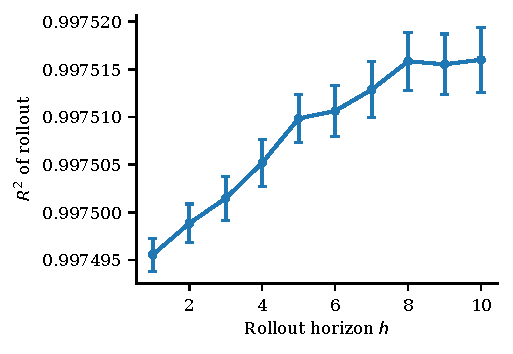
\includegraphics[width=\columnwidth]{figs/fig02_world_model.pdf}
\caption{Rollout $R^2$ versus horizon for the linear pilot model (mean, 95\% CI). Saturated; sanity check only.}
\label{fig:fig02_world_model}
\end{figure}

\section{Discussion and Limitations}
Simulated tasks are low-dimensional. Language goals are limited to a fixed set of instructions in this protocol. The linear probe measures recoverability of state, not sufficiency for control, which is why planning success is reported separately.

\section{Conclusion}
We outline a protocol that tests whether JEPA latents support planning, measured directly by simulator states and by task success under text-specified goals.

\section*{Acknowledgments}
The author thanks the Brazilian artificial intelligence community.

\nocite{ctl_full_names}
\bibliographystyle{IEEEtran}
\bibliography{refs}

\end{document}
